\begin{frame}{VLAN idea}
    \begin{itemize}
    \item multiple (`virtual') local networks over one network
    \item links/ports either shared or assigned to just one network
    \item most common implementation: Ethernt 802.1q:
    \vspace{.5cm}
    \item on shared links, frames tagged with their `VLAN ID'
        \begin{itemize}
        \item special case: untagged frames part of VLAN ID 0x0
        \end{itemize}
    \item tags added/removed when going to unshared links
        \begin{itemize}
        \item and broadcast frames filtered out if VLAN ID doesn't match
        \end{itemize}
    \end{itemize}
\end{frame}

\begin{frame}[fragile]{Ethernet encapsulation}
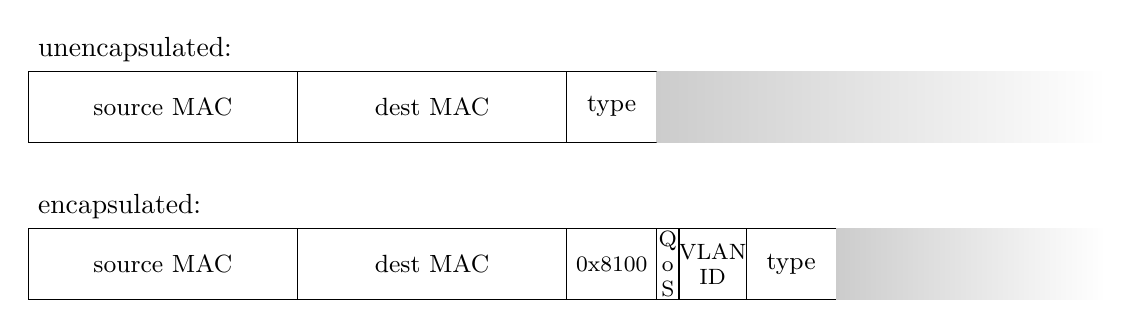
\begin{tikzpicture}
    \tikzset{
        box/.style={draw,thick},
        box unused/.style={draw,thick,pattern=north west lines},
        box label/.style={midway,font=\small,align=center},
        box label flags/.style={midway,font=\fontsize{8}{9}\selectfont,align=center},
        hi on/.style={alt=<#1>{ultra thick,fill=red!10}},
        explain box 1/.style={draw=red,line width=0.8mm,fill=white,anchor=center,at={(explain box loc 1)},align=center},
        explain box 2/.style={draw=red,line width=0.8mm,fill=white,anchor=center,at={(explain box loc 2)},align=center},
        explain box 3/.style={draw=red,line width=0.8mm,fill=white,anchor=center,at={(explain box loc 3)},align=center},
    }
    \begin{scope}[x=5.7mm,y=9mm]
        \node[anchor=south west] at (0, 0) {unencapsulated:};
        \coordinate (explain box loc 1) at (16, -6.1);
        \draw (0, 0) rectangle ++(6, -1) node[box label]{source MAC};
        \draw (6, 0) rectangle ++(6, -1) node[box label]{dest MAC};
        \draw (12, 0) rectangle ++(2, -1) node[box label]{type};
        \path[shading=axis,right color=white, left color=black!20] (14, 0) rectangle (24, -1);
    \end{scope}
    \begin{scope}[x=5.7mm,y=9mm,yshift=-2cm]
        \node[anchor=south west] at (0, 0) {encapsulated:};
        \draw (0, 0) rectangle ++(6, -1) node[box label]{source MAC};
        \draw (6, 0) rectangle ++(6, -1) node[box label]{dest MAC};
        \draw (12, 0) rectangle ++(2, -1) node[box label flags]{0x8100};
        \draw (14, 0) rectangle ++(.5, -1) node[box label flags]{Q\\o\\S};
        \draw (14.5, 0) rectangle ++(1.5, -1) node[box label flags]{VLAN\\ID};
        \draw (16, 0) rectangle ++(2, -1) node[box label]{type};
        \path[shading=axis,right color=white, left color=black!20] (18, 0) rectangle (24, -1);
    \end{scope}
\end{tikzpicture}
\begin{itemize}
    \item encapsulation typically added/removed by switches
        \begin{itemize}
        \item sysadmin configures specific ports to be on a VLAN
        \item another common case: virtual machine software
        \end{itemize}
    \item network IDs (`VLAN identifiers') configured by sysadmins
        \begin{itemize}
        \item special case: 0x0 = default (untagged), 0xFFF = reserved
        \end{itemize}
    \item usually increase in supported frame size to accomodate tag
\end{itemize}
\end{frame}

